\documentclass[10pt,a4paper]{article}
\usepackage[T1]{fontenc}
\usepackage[margin=2cm]{geometry}
\usepackage{isabelle,isabellesym}
\usepackage{amssymb}
\usepackage{tikz}
\usetikzlibrary{calc,arrows.meta}
\usepackage{float}
\usepackage{pdfsetup}

\urlstyle{rm}
\isabellestyle{it}

\begin{document}

\title{The Heilmann--Lieb Theorem: Real Roots of Matching Polynomials}
\author{Carles Mar\'in}
\maketitle

\begin{abstract}
The matching polynomial of a finite graph with $n$ vertices is
$\mu(G, x) = \sum_k (-1)^k m_k(G)\, x^{n-2k}$, where $m_k(G)$ is the number of matchings with $k$ edges.
Heilmann and Lieb proved in 1972 that all its roots are real. We formalize this theorem. The matching polynomial
satisfies the vertex recurrence $\mu(G) = x\,\mu(G-v) - \sum_{u \sim v} \mu(G-u-v)$, and the proof is an induction on
the number of vertices that keeps, besides real-rootedness, an interlacing property: for every vertex $v$,
$\mu(G-v)$ is a non-negative combination of the polynomials obtained from $\mu(G)$ by removing one linear factor.
This formulation handles repeated roots without any special treatment. Its analytic core is a lemma on real
polynomials, proved with the intermediate value theorem and Lagrange interpolation.
\end{abstract}

\paragraph{Acknowledgement.} The formalization and the text of this document were prepared with the
assistance of an AI system, and checked by the author.

\tableofcontents

\section*{Introduction}

A matching of a graph is a set of pairwise disjoint edges. The matching polynomial
$\mu(G, x) = \sum_M (-1)^{|M|} x^{n - 2|M|}$, the sum taken over all matchings $M$, appears in statistical physics as
the partition function of the monomer--dimer model, and Heilmann and Lieb~\cite{HeilmannLieb1972} proved that all its
roots are real; physically, the model has no phase transition. Godsil and Gutman~\cite{GodsilGutman1981} and
Godsil~\cite{Godsil1981} related it to the characteristic polynomial and to walks in graphs; a textbook account is
in~\cite{Godsil1993}.

We follow the interlacing route. Write $\mathrm{lin}(r_1, \ldots, r_m) = \prod_i (x - r_i)$ and say that a polynomial
$q$ lies in the \emph{cone} of the list $r_1, \ldots, r_m$ if $q = \sum_i c_i \prod_{j \neq i}(x - r_j)$ with all
$c_i \geq 0$. The induction (theory \texttt{Heilmann\_Lieb}) proves that $\mu(G) = \mathrm{lin}(r)$ for a list $r$
of real numbers and that $\mu(G - v)$ lies in the cone of $r$ for every vertex $v$. The step uses the recurrence
(theory \texttt{Matching\_Polynomial}) and one lemma on real polynomials (theory \texttt{Cone\_Step}): if $S$ lies in
the cone of $r$, then $x\,\mathrm{lin}(r) - S = \mathrm{lin}(t)$ for a list $t$ one element longer, and
$\mathrm{lin}(r)$ lies in the cone of $t$. To prove it, repeated roots of $r$ and roots with weight zero are taken
out as a common factor; for distinct roots $s_1 < \cdots < s_k$ with positive weights, the polynomial changes sign
between consecutive $s_j$ and at both ends, so the intermediate value theorem gives roots
$t_0 < s_1 < t_1 < \cdots < s_k < t_k$, and Lagrange interpolation at the $t_l$ writes $\mathrm{lin}(s)$ in their cone
with positive coefficients. Figure~\ref{fig:example} shows the interlacing for the 5-cycle, and
Figure~\ref{fig:roadmap} how the lemmas fit together.

% generated by research/frisos-sturm/figura_hl.py (Curiosity); do not edit by hand
\begin{figure}[H]
\centering
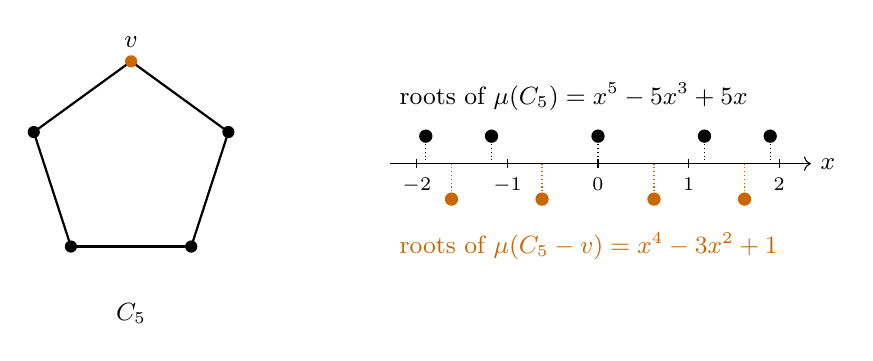
\begin{tikzpicture}[every node/.style={font=\small}]
  \draw[thick] (0.000,1.300) -- (-1.236,0.402);
  \draw[thick] (-1.236,0.402) -- (-0.764,-1.052);
  \draw[thick] (-0.764,-1.052) -- (0.764,-1.052);
  \draw[thick] (0.764,-1.052) -- (1.236,0.402);
  \draw[thick] (1.236,0.402) -- (0.000,1.300);
  \fill[fill=orange!80!black] (0.000,1.300) circle (2.2pt);
  \fill[fill=black] (-1.236,0.402) circle (2.2pt);
  \fill[fill=black] (-0.764,-1.052) circle (2.2pt);
  \fill[fill=black] (0.764,-1.052) circle (2.2pt);
  \fill[fill=black] (1.236,0.402) circle (2.2pt);
  \node[above] at (0.000,1.350) {$v$};
  \node at (0,-1.9) {$C_5$};
  \draw[->] (3.285,0) -- (8.633,0) node[right] {$x$};
  \draw (3.630,0.06) -- (3.630,-0.06) node[below] {\scriptsize $-2$};
  \draw (4.780,0.06) -- (4.780,-0.06) node[below] {\scriptsize $-1$};
  \draw (5.930,0.06) -- (5.930,-0.06) node[below] {\scriptsize $0$};
  \draw (7.080,0.06) -- (7.080,-0.06) node[below] {\scriptsize $1$};
  \draw (8.230,0.06) -- (8.230,-0.06) node[below] {\scriptsize $2$};
  \fill (3.743,0.35) circle (2.4pt);
  \draw[densely dotted] (3.743,0.35) -- (3.743,0);
  \fill (4.578,0.35) circle (2.4pt);
  \draw[densely dotted] (4.578,0.35) -- (4.578,0);
  \fill (5.930,0.35) circle (2.4pt);
  \draw[densely dotted] (5.930,0.35) -- (5.930,0);
  \fill (7.282,0.35) circle (2.4pt);
  \draw[densely dotted] (7.282,0.35) -- (7.282,0);
  \fill (8.117,0.35) circle (2.4pt);
  \draw[densely dotted] (8.117,0.35) -- (8.117,0);
  \fill[orange!80!black] (4.069,-0.45) circle (2.4pt);
  \draw[densely dotted, orange!80!black] (4.069,-0.45) -- (4.069,0);
  \fill[orange!80!black] (5.219,-0.45) circle (2.4pt);
  \draw[densely dotted, orange!80!black] (5.219,-0.45) -- (5.219,0);
  \fill[orange!80!black] (6.641,-0.45) circle (2.4pt);
  \draw[densely dotted, orange!80!black] (6.641,-0.45) -- (6.641,0);
  \fill[orange!80!black] (7.791,-0.45) circle (2.4pt);
  \draw[densely dotted, orange!80!black] (7.791,-0.45) -- (7.791,0);
  \node[anchor=west] at (3.285,0.85) {roots of $\mu(C_5) = x^5 - 5x^3 + 5x$};
  \node[anchor=west, orange!80!black] at (3.285,-1.05) {roots of $\mu(C_5 - v) = x^4 - 3x^2 + 1$};
\end{tikzpicture}
\caption{The matching polynomial of the 5-cycle and of the path obtained by deleting the vertex $v$: all roots are real (Theorem \texttt{heilmann\_lieb}) and they interlace, which is the cone property used in the induction. The roots are $0, \pm\sqrt{(5\pm\sqrt5)/2}$ and $\pm(\sqrt5\pm1)/2$.}
\label{fig:example}
\end{figure}


% Roadmap of the proof (names as in the theories).
\begin{figure}[H]
\centering
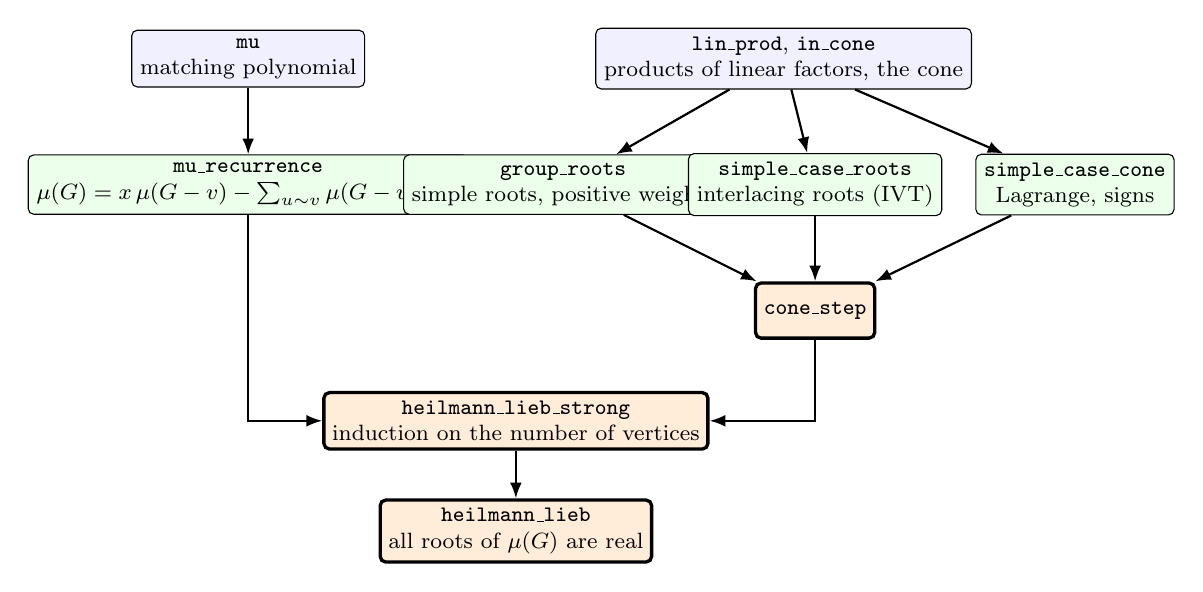
\begin{tikzpicture}[
    box/.style={draw, rounded corners=2pt, align=center, font=\footnotesize, inner sep=3pt, minimum height=7mm},
    def/.style={box, fill=blue!6},
    lem/.style={box, fill=green!8},
    thm/.style={box, fill=orange!15, very thick},
    arr/.style={-{Latex[length=2mm]}, thick}]
  \node[def] (mu)  at (-4.6,0)    {\texttt{mu}\\ matching polynomial};
  \node[lem] (rec) at (-4.6,-1.6) {\texttt{mu\_recurrence}\\ $\mu(G) = x\,\mu(G-v) - \sum_{u\sim v}\mu(G-u-v)$};
  \node[def] (cone) at (2.2,0)    {\texttt{lin\_prod}, \texttt{in\_cone}\\ products of linear factors, the cone};
  \node[lem] (grp) at (-0.6,-1.6) {\texttt{group\_roots}\\ simple roots, positive weights};
  \node[lem] (scr) at (2.6,-1.6)  {\texttt{simple\_case\_roots}\\ interlacing roots (IVT)};
  \node[lem] (scc) at (5.9,-1.6)  {\texttt{simple\_case\_cone}\\ Lagrange, signs};
  \node[thm] (cs)  at (2.6,-3.2)  {\texttt{cone\_step}};
  \node[thm] (hls) at (-1.2,-4.6) {\texttt{heilmann\_lieb\_strong}\\ induction on the number of vertices};
  \node[thm] (hl)  at (-1.2,-6.0) {\texttt{heilmann\_lieb}\\ all roots of $\mu(G)$ are real};
  \draw[arr] (mu) -- (rec);
  \draw[arr] (cone) -- (grp);
  \draw[arr] (cone) -- (scr);
  \draw[arr] (cone) -- (scc);
  \draw[arr] (grp) -- (cs);
  \draw[arr] (scr) -- (cs);
  \draw[arr] (scc) -- (cs);
  \draw[arr] (rec.south) |- (hls.west);
  \draw[arr] (cs.south) |- (hls.east);
  \draw[arr] (hls) -- (hl);
\end{tikzpicture}
\caption{How the main lemmas lead to the theorem. Blue: definitions; green: lemmas; orange: the main results.}
\label{fig:roadmap}
\end{figure}


\parindent 0pt\parskip 0.5ex

\input{session}

\bibliographystyle{abbrv}
\bibliography{root}

\end{document}
